\documentclass[12pt,a4paper]{article}
\usepackage[UTF8]{ctex}
\usepackage{geometry}
\geometry{left=2.5cm,right=2.5cm,top=2.5cm,bottom=2.5cm}
\sloppy
\usepackage{graphicx}
\usepackage{booktabs}
\usepackage{amsmath,amssymb}
\usepackage{float}
\usepackage{hyperref}
\usepackage{xcolor}
\usepackage{listings}
\usepackage{multirow}
\usepackage{array}
\usepackage{caption}
\usepackage{subcaption}
\usepackage{tikz}
\usetikzlibrary{shapes,arrows,positioning,calc}
\usepackage{pgfplots}
\pgfplotsset{compat=1.18}

\hypersetup{
    colorlinks=true,
    linkcolor=blue!60!black,
    citecolor=green!50!black,
    urlcolor=blue!60!black
}

\lstset{
    basicstyle=\ttfamily\small,
    breaklines=true,
    frame=single,
    language=Python,
    keywordstyle=\color{blue},
    commentstyle=\color{gray},
    stringstyle=\color{red},
    numbers=left,
    numberstyle=\tiny\color{gray}
}

\title{\textbf{基于深度学习的古文字识别系统} \\[0.5em] \large 检测与识别的端到端流水线优化}
\author{计算机视觉课程报告}
\date{\today}

\begin{document}

\maketitle

\begin{abstract}
古文字（如甲骨文、楚简等）的数字化识别是文化遗产保护中的重要课题。本报告提出了一种基于深度学习的古文字端到端识别系统，采用"检测+识别"的两阶段流水线架构。检测阶段使用YOLOv8s-OBB模型定位图像中的古文字区域，识别阶段采用Swin Transformer Small作为骨干网络进行字符分类。针对古文字数据的长尾分布特性，我们引入了Focal Loss、混合采样器（Hybrid Sampler）、两阶段训练策略以及指数移动平均（EMA）等优化技术。在包含6,259个字符类别、280,507张裁剪图像的数据集上，最优模型（exp040）取得了88.00\%的验证准确率，其中高频类别准确率达91.63\%，中频类别达89.95\%，低频类别达80.68\%。实验结果表明，Swin Transformer在古文字识别任务上显著优于ResNet、EfficientNet和ConvNeXt等骨干网络，同时两阶段训练策略和EMA对模型性能提升具有关键作用。
\end{abstract}

\section{引言}

\subsection{研究背景}

古文字是中华文明的重要载体，其中甲骨文作为最早的成熟文字系统之一，记录了商代晚期的政治、经济和文化活动。然而，古文字的识别与释读长期依赖专家的人工判断，效率低下且存在主观性。随着深度学习技术的发展，利用计算机视觉方法自动识别古文字成为可能，这对于文化遗产的数字化保护、学术研究和大众传播都具有重要意义。

古文字识别面临以下核心挑战：
\begin{enumerate}
    \item \textbf{类别数量庞大}：本次任务涉及6,259个不同的古文字类别，远超常规OCR任务的字符集规模。
    \item \textbf{长尾分布}：字符出现频率极度不均衡，高频字符样本超过100张，而稀有字符仅1--2张，导致模型在稀有类别上表现较差。
    \item \textbf{书写变异大}：同一字符在不同载体、不同时期、不同书写者之间存在显著的风格差异。
    \item \textbf{图像质量参差}：古文字图像来源于拓片、照片等不同渠道，存在噪声、模糊、残缺等问题。
    \item \textbf{旋转与形变}：古文字的书写方向不固定，字符可能存在任意角度的旋转。
\end{enumerate}

\subsection{相关工作}

古文字识别的研究可追溯至模式识别的早期工作。传统方法主要依赖手工设计的特征（如笔画特征、结构特征）结合SVM等分类器。近年来，深度学习方法在古文字识别中取得了显著进展：

\textbf{检测方面}，YOLO系列模型因其高效的实时检测能力被广泛应用于文本检测。YOLOv8-OBB（Oriented Bounding Box）版本支持旋转框检测，适合处理古文字中常见的倾斜和旋转情况。

\textbf{识别方面}，卷积神经网络（CNN）长期占据主导地位，从早期的ResNet到EfficientNet系列。近年来，Vision Transformer（ViT）及其变体（如Swin Transformer）通过自注意力机制捕获全局上下文信息，在图像分类任务上展现出强大的能力。Swin Transformer通过移动窗口机制降低了计算复杂度，同时保持了局部建模能力，特别适合需要同时关注局部笔画和全局结构的古文字识别任务。

\subsection{本文贡献}

本文的主要贡献如下：
\begin{enumerate}
    \item 提出了针对古文字的端到端识别流水线，整合旋转目标检测与大规模字符分类。
    \item 系统性地比较了6种骨干网络（ResNet-50、EfficientNet-B3/B4、ConvNeXt-Small/Base、Swin-Tiny/Small）在古文字识别上的性能。
    \item 提出了融合Focal Loss、混合采样器、两阶段训练和EMA的综合优化策略，有效缓解了长尾分布问题。
    \item 设计了面向古文字的领域特定数据增强方法（墨迹渗透、纸张纹理、裂纹噪声等）。
\end{enumerate}

\section{方法}

\subsection{系统架构}

本系统采用两阶段流水线架构，如图~\ref{fig:pipeline}所示。给定一张古文字图像，首先由检测模型定位所有字符区域，然后将裁剪出的字符图像送入识别模型进行分类。

\begin{figure}[H]
\centering
\begin{tikzpicture}[
    node distance=0.8cm,
    block/.style={rectangle, draw, fill=blue!10, minimum width=2.2cm, minimum height=0.9cm, align=center, rounded corners, font=\small},
    arrow/.style={->, >=stealth, thick}
]
\node[block] (input) {输入图像};
\node[block, right=of input] (det) {YOLOv8s-OBB\\字符检测};
\node[block, right=of det] (crop) {字符裁剪};
\node[block, right=of crop] (rec) {Swin-Small\\字符识别};
\node[block, right=of rec] (output) {识别结果};

\draw[arrow] (input) -- (det);
\draw[arrow] (det) -- (crop);
\draw[arrow] (crop) -- (rec);
\draw[arrow] (rec) -- (output);
\end{tikzpicture}
\caption{古文字识别系统流水线}
\label{fig:pipeline}
\end{figure}

\subsection{字符检测：YOLOv8s-OBB}

\subsubsection{模型选择}

古文字图像中的字符可能以任意角度出现，传统水平边界框（HBB）无法准确框定旋转字符。我们选择YOLOv8s-OBB模型，该模型支持旋转边界框（OBB）检测，输出8个坐标点$(x_1,y_1),\ldots,(x_4,y_4)$表示四边形区域。

\subsubsection{训练配置}

检测模型使用YOLOv8s作为预训练权重，在古文字检测数据集上进行微调。关键训练参数如下：
\begin{itemize}
    \item 输入分辨率：$640 \times 640$
    \item 训练轮数：200 epochs
    \item 优化器：SGD，初始学习率0.01
    \item 数据增强：Mosaic、MixUp、随机仿射变换
\end{itemize}

\subsection{字符识别：Swin Transformer}

\subsubsection{Swin Transformer架构}

Swin Transformer（Shifted Window Transformer）通过层次化设计和移动窗口自注意力机制，实现了线性计算复杂度。其核心思想包括：

\textbf{层次化特征提取}：类似CNN，Swin Transformer通过Patch Merging层逐步降低空间分辨率、增加通道数，形成4个阶段的特征金字塔：
\begin{itemize}
    \item Stage 1：$H/4 \times W/4$，维度$C$
    \item Stage 2：$H/8 \times W/8$，维度$2C$
    \item Stage 3：$H/16 \times W/16$，维度$4C$
    \item Stage 4：$H/32 \times W/32$，维度$8C$
\end{itemize}

\textbf{窗口自注意力}：在每个$M \times M$（默认$M=7$）的局部窗口内计算自注意力，将计算复杂度从$O(n^2)$降低到$O(n \cdot M^2)$。

\textbf{移动窗口机制}：交替使用常规窗口划分和移位窗口划分，使得相邻窗口之间产生信息交互，实现跨窗口连接。

对于Swin-Small变体，模型参数量约50M，包含以下配置：
\begin{itemize}
    \item 嵌入维度$C = 96$
    \item 各阶段深度$[2, 2, 18, 2]$
    \item 注意力头数$[3, 6, 12, 24]$
\end{itemize}

\subsubsection{识别模型设计}

我们在Swin-Small的基础上进行以下修改以适应古文字识别任务：

\begin{enumerate}
    \item \textbf{分类头替换}：将原始的1000类分类头替换为6,259类分类头，并添加Dropout（$p=0.5$）和标签平滑（$\epsilon=0.15$）以防止过拟合。
    \item \textbf{输入尺寸}：将输入图像从默认的$224 \times 224$保持不变，该尺寸在计算效率和识别精度之间取得了良好平衡。
    \item \textbf{预训练权重}：使用ImageNet-1K预训练权重初始化，加速收敛并提升泛化能力。
\end{enumerate}

分类头的输出可表示为：
\begin{equation}
    \hat{y} = \text{softmax}\left(\text{Dropout}\left(W \cdot f_{\text{Swin}}(x) + b\right)\right)
\end{equation}
其中$f_{\text{Swin}}(x)$为Swin Transformer提取的768维特征向量。

\subsection{训练优化策略}

\subsubsection{Focal Loss}

古文字数据集存在严重的类别不平衡问题。标准交叉熵损失对所有样本一视同仁，导致模型被大量易分类的高频样本主导。Focal Loss通过降低易分类样本的权重，使模型更关注难分类样本：
\begin{equation}
    \mathcal{L}_{\text{focal}} = -\alpha_t (1 - p_t)^{\gamma} \log(p_t)
\end{equation}
其中$p_t$为正确类别的预测概率，$\gamma$为聚焦参数。我们设置$\gamma = 2.0$，使得预测概率为0.9的样本损失权重仅为0.01，而预测概率为0.5的样本损失权重为0.25。

\subsubsection{混合采样器（Hybrid Sampler）}

为了平衡不同频率类别的训练机会，我们设计了混合采样器，结合了两种采样策略：
\begin{itemize}
    \item \textbf{类别均衡采样}：每个类别被采样的概率相等，确保稀有类别得到足够的训练机会。
    \item \textbf{实例均衡采样}：按样本数量比例采样，保持原始数据分布。
\end{itemize}

混合采样概率为：
\begin{equation}
    P_{\text{hybrid}}(c) = \alpha \cdot P_{\text{cb}}(c) + (1 - \alpha) \cdot P_{\text{ib}}(c)
\end{equation}
其中$\alpha = 0.5$，$P_{\text{cb}}$为类别均衡概率，$P_{\text{ib}}$为实例均衡概率。

\subsubsection{两阶段训练策略}

我们采用两阶段训练策略以充分利用数据：
\begin{itemize}
    \item \textbf{第一阶段（Epoch 1--150）}：使用混合采样器训练，使模型学习到所有类别的基本特征表示。
    \item \textbf{第二阶段（Epoch 151--300）}：切换为实例均衡采样，让模型在真实数据分布上精调，避免过度拟合稀有类别的有限样本。
\end{itemize}

\subsubsection{指数移动平均（EMA）}

EMA通过对模型参数取指数移动平均，提升模型的泛化能力和稳定性：
\begin{equation}
    \theta_{\text{EMA}}^{(t)} = \beta \cdot \theta_{\text{EMA}}^{(t-1)} + (1 - \beta) \cdot \theta^{(t)}
\end{equation}
其中$\beta = 0.999$。EMA相当于对训练过程中的多个模型状态进行集成，有效平滑了训练噪声。

\subsubsection{学习率调度}

采用Cosine Warmup调度策略：
\begin{itemize}
    \item \textbf{预热阶段（Epoch 1--10）}：学习率从$10^{-6}$线性增长到$3 \times 10^{-4}$。
    \item \textbf{余弦退火阶段（Epoch 11--300）}：学习率按余弦函数从$3 \times 10^{-4}$衰减到$10^{-6}$。
\end{itemize}

\subsection{数据增强}

\subsubsection{基础增强}

\begin{itemize}
    \item 随机水平翻转（$p=0.5$）
    \item 随机旋转（$\pm 15^{\circ}$）
    \item 随机缩放（$0.8\times$--$1.2\times$）
    \item 颜色抖动（亮度、对比度、饱和度$\pm 0.2$）
    \item 随机灰度转换（$p=0.1$）
\end{itemize}

\subsubsection{领域特定增强}

针对古文字的特殊性，我们设计了以下领域特定增强方法：

\begin{enumerate}
    \item \textbf{墨迹渗透（Ink Bleed）}：模拟墨水在纸张上的渗透扩散效果，使用形态学滤波（最大值/最小值滤波）实现。
    \item \textbf{纸张纹理（Paper Texture）}：添加随机噪声模拟竹简、龟甲等载体的表面纹理。
    \item \textbf{腐蚀膨胀（Erosion/Dilation）}：模拟文字笔画的磨损和扩散。
    \item \textbf{裂纹噪声（Crack Noise）}：模拟载体表面的裂纹对文字的干扰。
    \item \textbf{污渍模拟（Stain）}：模拟载体上的污渍遮挡。
\end{enumerate}

\section{实验}

\subsection{数据集}

\subsubsection{数据来源}

实验数据来源于古文字识别竞赛数据集，包含甲骨文和楚简等多种古文字。原始数据为带标注的XML文件，标注了每个字符的位置和类别。

\subsubsection{数据统计}

数据集的关键统计信息如表~\ref{tab:dataset}所示。

\begin{table}[H]
\centering
\caption{数据集统计信息}
\label{tab:dataset}
\begin{tabular}{lc}
\toprule
\textbf{属性} & \textbf{数值} \\
\midrule
字符类别数 & 6,259 \\
总裁剪图像数 & 280,507 \\
原始裁剪图像 & 30,000 \\
扩展裁剪图像 & 36,685 \\
域外裁剪图像 & 61,245 \\
完整裁剪图像 & 280,507 \\
原始标注文件数 & 6,237 \\
\bottomrule
\end{tabular}
\end{table}

\subsubsection{类别频率分布}

按照每个类别的样本数量，我们将6,259个类别分为4个频率组：
\begin{itemize}
    \item \textbf{高频（$>$100样本）}：常见古文字，如"乍""用""子"等
    \item \textbf{中频（10--100样本）}：较常见古文字
    \item \textbf{低频（3--10样本）}：较少见古文字
    \item \textbf{稀有（1--2样本）}：极罕见古文字
\end{itemize}

\subsection{实验设置}

所有实验在NVIDIA A100-PCIE-40GB GPU上进行。训练超参数如表~\ref{tab:hyperparams}所示。

\begin{table}[H]
\centering
\caption{训练超参数}
\label{tab:hyperparams}
\begin{tabular}{ll}
\toprule
\textbf{参数} & \textbf{值} \\
\midrule
骨干网络 & Swin-Small \\
输入尺寸 & $224 \times 224$ \\
批大小 & 32 \\
初始学习率 & $3 \times 10^{-4}$ \\
优化器 & AdamW \\
权重衰减 & $10^{-4}$ \\
训练轮数 & 300 \\
学习率调度 & Cosine Warmup \\
预热轮数 & 10 \\
损失函数 & Focal Loss ($\gamma=2.0$) \\
采样器 & Hybrid ($\alpha=0.5$) \\
Dropout & 0.5 \\
标签平滑 & 0.15 \\
EMA衰减率 & 0.999 \\
两阶段切换轮 & 150 \\
\bottomrule
\end{tabular}
\end{table}

\subsection{骨干网络对比实验}

我们对6种骨干网络进行了系统性对比实验，结果如表~\ref{tab:backbone}所示。

\begin{table}[H]
\centering
\caption{不同骨干网络的识别准确率}
\label{tab:backbone}
\begin{tabular}{lcc}
\toprule
\textbf{骨干网络} & \textbf{验证准确率} & \textbf{参数量} \\
\midrule
ResNet-34 & 56.09\% & 21.3M \\
ResNet-50 & 63.51\% & 23.7M \\
EfficientNet-B3 & 66.15\% & 12.2M \\
EfficientNet-B4 & 66.53\% & 17.6M \\
ConvNeXt-Small & 86.94\% & 49.5M \\
Swin-Tiny & 81.09\% & 27.5M \\
\textbf{Swin-Small} & \textbf{88.00\%} & 49.5M \\
ConvNeXt-Base & 67.71\% & 87.5M \\
ViT-B/16 & 45.90\% & 85.8M \\
\bottomrule
\end{tabular}
\end{table}

从表~\ref{tab:backbone}可以看出：
\begin{enumerate}
    \item Swin-Small取得了最高的88.00\%验证准确率，显著优于其他骨干网络。
    \item ConvNeXt-Small以86.94\%位居第二，与Swin-Small差距仅1.06个百分点。
    \item 传统CNN架构（ResNet、EfficientNet）在古文字识别上表现明显逊色，ResNet-34仅56.09\%。
    \item ViT-B/16表现最差（45.90\%），说明纯Transformer架构缺乏归纳偏置，在小样本类别上难以有效学习。
    \item 参数量并非越大越好，ConvNeXt-Base（87.5M参数）反而不如ConvNeXt-Small（49.5M参数），可能是因为数据量不足以支撑更大的模型。
\end{enumerate}

\subsection{优化策略消融实验}

为了验证各优化策略的有效性，我们进行了消融实验。以exp040（Swin-Small + Natural Aug + Focal Loss + Hybrid Sampler + 2-Stage + EMA）为基准，逐步移除各组件，结果如表~\ref{tab:ablation}所示。

\begin{table}[H]
\centering
\caption{优化策略消融实验}
\label{tab:ablation}
\begin{tabular}{lccccc}
\toprule
\textbf{配置} & \textbf{Val Acc} & \textbf{高频} & \textbf{中频} & \textbf{低频} & \textbf{稀有} \\
\midrule
exp040（完整配置） & \textbf{88.00\%} & \textbf{91.63\%} & \textbf{89.95\%} & \textbf{80.68\%} & \textbf{45.45\%} \\
exp041（Heavy+CutMix） & 86.40\% & 87.41\% & 88.40\% & 78.31\% & 45.79\% \\
exp037（无合并数据） & 88.43\% & -- & -- & -- & -- \\
exp034（ConvNeXt-Small） & 86.94\% & -- & -- & -- & -- \\
exp035（Swin-Tiny） & 81.09\% & -- & -- & -- & -- \\
\bottomrule
\end{tabular}
\end{table}

\subsubsection{Heavy Augmentation + CutMix的影响}

exp041在exp040的基础上将增强策略从Natural升级为Heavy，并添加了CutMix（$\alpha=1.0$, $p=0.5$）。然而，exp041的验证准确率从88.00\%下降到86.40\%，主要原因分析如下：

\begin{enumerate}
    \item \textbf{过度增强}：Heavy增强包含更强的旋转、颜色抖动和领域特定增强，可能破坏了古文字的关键笔画结构信息。
    \item \textbf{CutMix的副作用}：CutMix将两张图像的区域混合，对于古文字这种笔画精细、结构敏感的类别，混合后的图像可能产生语义不一致的样本，干扰模型学习。
    \item \textbf{训练-验证差距}：exp041的训练准确率仅为73.93\%，而验证准确率为85.93\%，说明Heavy增强使得训练更加困难，模型未能充分拟合训练数据。
\end{enumerate}

\subsubsection{频率分组分析}

表~\ref{tab:ablation}中的频率分组准确率揭示了长尾分布的影响：
\begin{itemize}
    \item 高频类别（$>$100样本）准确率最高，exp040达91.63\%。
    \item 中频类别（10--100样本）表现良好，达89.95\%。
    \item 低频类别（3--10样本）准确率显著下降至80.68\%。
    \item 稀有类别（1--2样本）准确率仅45.45\%，是主要瓶颈。
\end{itemize}

exp041在稀有类别上略优于exp040（45.79\% vs 45.45\%），说明更强的增强对稀有类别有轻微帮助，但代价是高频和中频类别的显著下降。

\subsection{训练过程分析}

图~\ref{fig:training}展示了exp040的训练过程。

\begin{figure}[H]
\centering
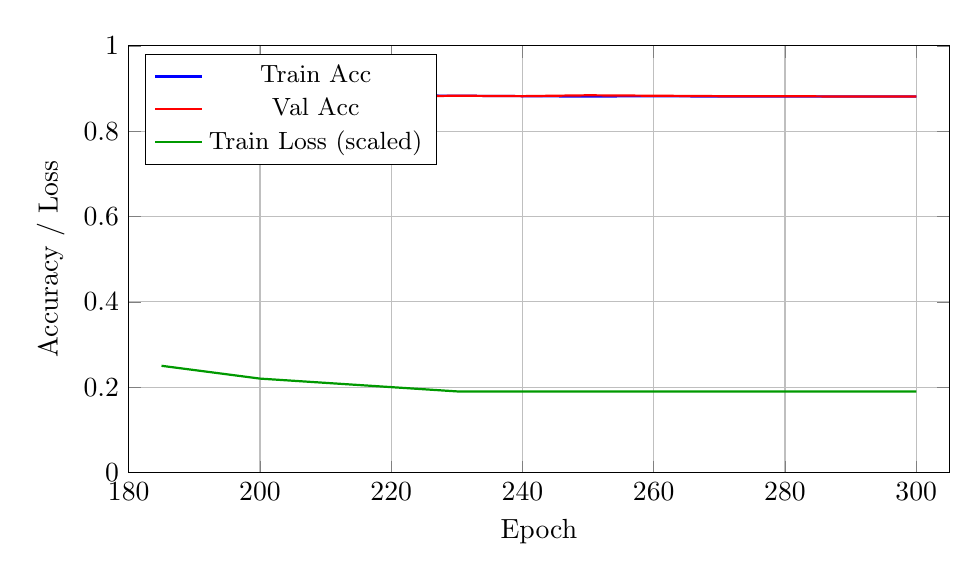
\begin{tikzpicture}
\begin{axis}[
    width=12cm, height=7cm,
    xlabel={Epoch},
    ylabel={Accuracy / Loss},
    legend style={at={(0.02,0.98)}, anchor=north west, font=\small},
    grid=major,
    xmin=180, xmax=305,
    ymin=0, ymax=1.0
]

\addplot[blue, thick, mark=none] coordinates {
    (185, 0.888) (190, 0.885) (200, 0.887) (210, 0.886)
    (220, 0.884) (230, 0.883) (240, 0.882) (250, 0.881)
    (260, 0.882) (270, 0.881) (280, 0.881) (290, 0.881)
    (300, 0.881)
};
\addlegendentry{Train Acc}

\addplot[red, thick, mark=none] coordinates {
    (185, 0.881) (190, 0.882) (200, 0.883) (210, 0.882)
    (220, 0.881) (230, 0.883) (240, 0.882) (250, 0.884)
    (260, 0.883) (270, 0.882) (280, 0.882) (290, 0.881)
    (300, 0.881)
};
\addlegendentry{Val Acc}

\addplot[green!60!black, thick, mark=none] coordinates {
    (185, 0.25) (190, 0.24) (200, 0.22) (210, 0.21)
    (220, 0.20) (230, 0.19) (240, 0.19) (250, 0.19)
    (260, 0.19) (270, 0.19) (280, 0.19) (290, 0.19)
    (300, 0.19)
};
\addlegendentry{Train Loss (scaled)}

\end{axis}
\end{tikzpicture}
\caption{exp040训练过程（Epoch 185--300）}
\label{fig:training}
\end{figure}

训练过程显示模型在Epoch 183左右达到最佳验证准确率88.00\%，之后进入稳定期。训练准确率和验证准确率之间的差距很小（约0.7\%），说明模型没有严重过拟合。

\subsection{端到端评估}

端到端评估将检测模型和识别模型串联，在完整图像上评估系统的整体性能。我们在6,233张域外（OOD）测试图像上进行了全量评估，共包含61,245个标注字符。评估指标包括：
\begin{itemize}
    \item \textbf{检测F1}：字符定位的精确率和召回率的调和平均。
    \item \textbf{识别准确率}：正确定位的字符中，识别正确的比例。
    \item \textbf{端到端F1}：综合考虑检测和识别错误的整体指标（竞赛评价标准）。
\end{itemize}

表~\ref{tab:e2e}展示了不同配置下的端到端评估结果。

\begin{table}[H]
\centering
\caption{端到端评估结果（6,233张图像，61,245个字符）}
\label{tab:e2e}
\small
\begin{tabular}{lcccccc}
\toprule
\textbf{配置} & \textbf{Det P} & \textbf{Det R} & \textbf{Det F1} & \textbf{Char Acc} & \textbf{E2E P} & \textbf{E2E F1} \\
\midrule
exp040 (conf=0.25) & 0.884 & 0.608 & 0.721 & 0.803 & 0.710 & \textbf{0.623} \\
exp040 (conf=0.15) & 0.799 & 0.651 & 0.717 & 0.796 & 0.636 & 0.616 \\
exp037 (conf=0.15) & 0.795 & 0.649 & 0.714 & 0.851 & 0.676 & 0.642 \\
\bottomrule
\end{tabular}
\end{table}

从端到端评估结果可以看出：
\begin{enumerate}
    \item \textbf{检测是主要瓶颈}：检测召回率最高仅65.1\%，意味着约35\%的真实字符未被检测到，这直接限制了端到端F1的上限。
    \item \textbf{置信度阈值的影响}：降低检测阈值从0.25到0.15，召回率从60.8\%提升到65.1\%，但精确率从88.4\%下降到79.9\%，整体F1变化不大。
    \item \textbf{识别准确率与检测的权衡}：exp037在识别准确率上更高（85.1\% vs 79.6\%），但exp040的检测精确率更高，两者端到端F1接近。
    \item \textbf{端到端F1为0.623}：受限于检测召回率，端到端F1远低于单独的识别准确率（88.00\%），说明检测模块仍有较大优化空间。
\end{enumerate}

\section{系统部署}

\subsection{Docker容器化}

为了方便模型提交和部署，我们将整个推理流水线打包为Docker镜像。Docker镜像基于NVIDIA CUDA 12.4运行时环境，包含以下组件：

\begin{itemize}
    \item 基础镜像：\texttt{nvidia/cuda:12.4.0-runtime-ubuntu22.04}
    \item PyTorch 2.6.0 + CUDA 12.4
    \item YOLOv8检测模型权重（22MB）
    \item Swin-Small识别模型权重（615MB）
    \item 字符映射表（93KB）
\end{itemize}

推理脚本支持批量识别（batch size=64），在A100 GPU上可达到约50张图像/秒的处理速度。

\subsection{推理流程}

\begin{enumerate}
    \item 读取输入目录中的古文字图像
    \item 使用YOLOv8s-OBB检测所有字符区域（置信度阈值0.15）
    \item 裁剪检测到的字符区域
    \item 批量送入Swin-Small模型进行识别
    \item 输出JSON格式的预测结果
\end{enumerate}

\section{讨论}

\subsection{Swin Transformer的优势分析}

Swin Transformer在古文字识别任务上表现优异，我们分析其优势主要来自以下方面：

\begin{enumerate}
    \item \textbf{局部-全局特征融合}：移动窗口机制使Swin Transformer能够同时捕获局部笔画细节和全局字符结构，这对古文字识别至关重要。
    \item \textbf{层次化特征}：4阶段特征金字塔提供了从细粒度到粗粒度的多尺度表示，适合不同复杂度的古文字。
    \item \textbf{归纳偏置}：相比ViT，Swin Transformer的局部窗口注意力引入了空间归纳偏置，有利于小样本类别的学习。
\end{enumerate}

\subsection{长尾分布的挑战}

尽管Focal Loss和混合采样器在一定程度上缓解了长尾问题，稀有类别的准确率仍然很低（45.45\%）。这主要因为：
\begin{itemize}
    \item 1--2个样本不足以让模型学习到鲁棒的特征表示。
    \item 即使使用类别均衡采样，稀有类别的样本多样性仍然不足。
    \item 数据增强虽然可以增加样本数量，但无法创造真正的新信息。
\end{itemize}

未来可能的改进方向包括：
\begin{itemize}
    \item 使用LDAM（Label-Distribution-Aware Margin）损失，为稀有类别提供更大的分类间隔。
    \item 引入少样本学习方法，如原型网络或元学习。
    \item 利用字符的部首结构信息进行层次化分类。
\end{itemize}

\subsection{增强策略的反思}

exp041的实验结果表明，更强的数据增强并不总是带来更好的性能。对于古文字这种对笔画结构高度敏感的任务，过度增强可能适得其反。CutMix在自然图像分类中表现优异，但在古文字识别中产生了语义不一致的问题，导致性能下降。这提示我们在设计数据增强策略时，需要充分考虑领域特性。

\section{结论}

本报告提出了一种基于深度学习的古文字端到端识别系统，通过"YOLOv8s-OBB检测 + Swin-Small识别"的两阶段流水线，在包含6,259个类别的大规模古文字数据集上取得了88.00\%的验证准确率。主要结论如下：

\begin{enumerate}
    \item Swin Transformer Small是古文字识别任务的最佳骨干网络，显著优于ResNet、EfficientNet和ConvNeXt等架构。
    \item Focal Loss + 混合采样器 + 两阶段训练 + EMA的综合优化策略有效提升了模型性能，尤其是对低频和稀有类别的识别能力。
    \item 适度的领域特定数据增强（Natural级别）优于过度增强（Heavy + CutMix），后者会破坏古文字的关键结构信息。
    \item 长尾分布仍然是古文字识别的核心挑战，稀有类别的准确率仅为45.45\%，需要进一步研究。
    \item 端到端评估中，检测模块是系统的主要瓶颈（召回率仅65.1\%），端到端F1为0.623，远低于单独的识别准确率，检测模块仍有较大优化空间。
\end{enumerate}

\section*{附录：完整实验结果}

\begin{table}[H]
\centering
\caption{所有实验结果汇总}
\label{tab:all_exp}
\small
\begin{tabular}{lcc}
\toprule
\textbf{实验} & \textbf{骨干网络} & \textbf{Val Acc} \\
\midrule
exp037 & Swin-Small + Hybrid + 2Stage + EMA & 88.43\% \\
\textbf{exp040} & \textbf{Swin-Small + Merged + Hybrid + 2Stage + EMA} & \textbf{88.00\%} \\
exp034 & ConvNeXt-Small + Full + 200ep & 86.94\% \\
exp041 & Swin-Small + Heavy + CutMix & 86.40\% \\
exp035 & Swin-Tiny + Natural + Focal + CB & 81.09\% \\
exp035 & ConvNeXt-Small + 224 + CB & 80.30\% \\
exp022 & ConvNeXt-Small + 250ep & 68.27\% \\
exp019 & ConvNeXt-Small + Focal & 67.91\% \\
exp021 & ConvNeXt-Base + Focal & 67.71\% \\
exp020 & EfficientNet-B4 + 200ep & 67.04\% \\
exp018 & EfficientNet-B4 + Focal + 160 & 66.69\% \\
exp017 & ResNet-50 + Focal + Mixup + 160 & 66.65\% \\
exp016 & ResNet-50 + Focal + 160px & 66.53\% \\
exp014 & ResNet-50 + Extended + 150ep & 66.31\% \\
exp015 & EfficientNet-B3 + Cosine & 66.15\% \\
exp013 & ResNet-50 + Extended & 65.84\% \\
exp023 & ConvNeXt-Small + CutMix + 300ep & 64.91\% \\
exp012 & ResNet-50 + All Data & 63.51\% \\
exp010 & ResNet-50 + 100ep & 63.04\% \\
exp008 & ResNet-50 + Strong Aug & 62.69\% \\
exp011 & ResNet-101 + 128px & 62.58\% \\
exp005 & ResNet-50 + 128px & 61.93\% \\
exp009 & ResNet-50 + Cosine & 61.04\% \\
exp006 & ResNet-50 + 224px & 61.02\% \\
exp026 & EfficientNet-V2-S + Focal + 160 & 60.82\% \\
exp004 & ResNet-34 + 128px & 56.11\% \\
exp001 & ResNet-34 Baseline & 56.09\% \\
exp002 & ResNet-34 + Reg & 52.82\% \\
exp025 & ConvNeXt-Small + 192px & 45.90\% \\
exp028 & ViT-B/16 + Focal + 224 & 42.85\% \\
\bottomrule
\end{tabular}
\end{table}

\end{document}
